% Pre-ambulo
\documentclass[a4paper, 12pt]{abnt}

%% Pacotes para texto em Ingl�s
% \usepackage[brazil]{babel}
% \usepackage[T1]{fontenc}
% \usepackage[latin1]{inputenc}
 
%% Pacotes para texto em Portugues
\usepackage[brazil]{babel}
\usepackage[utf8]{inputenc}
\usepackage[T1]{fontenc}
\usepackage[labelfont=bf]{caption}
 
\usepackage{dsfont}
\usepackage{amssymb,amsmath}
\usepackage{multirow}
\usepackage[alf]{abntcite}
\usepackage[pdftex]{color, graphicx}
\usepackage{colortbl} 
\usepackage{url}
\usepackage{abnt-alf}
\usepackage{abntcite}
% \usepackage{algorithm}
% \usepackage{algorithmic}
% \usepackage{algorithm2e}
\usepackage[vlined,linesnumbered, portuguese, onelanguage]{algorithm2e}
% \usepackage{alg} 
%\usepackage{hyperref}



% Redefinicao de instrucoes
% \floatname{algorithm}{Algoritmo}
% \renewcommand{\algorithmicrequire}{\textbf{Entrada:}}
% \renewcommand{\algorithmicensure}{\textbf{Saida:}}
% \renewcommand{\algorithmicend}{\textbf{fim}}
% \renewcommand{\algorithmicif}{\textbf{se}}
% \renewcommand{\algorithmicthen}{\textbf{entao}}
% \renewcommand{\algorithmicelse}{\textbf{senaoo}}
% \renewcommand{\algorithmicfor}{\textbf{para}}
% \renewcommand{\algorithmicforall}{\textbf{para todo}}
% \renewcommand{\algorithmicdo}{\textbf{faca}}
% \renewcommand{\algorithmicwhile}{\textbf{enquanto}}
% \renewcommand{\algorithmicloop}{\textbf{loop}}
% \renewcommand{\algorithmicrepeat}{\textbf{repetir}}
% \renewcommand{\algorithmicuntil}{\textbf{ate que}}
% \renewcommand{\algorithmiccomment}[1]{\% #1}


% Definicao da lista de simbolos
% \simb[entrada na lista de simbolos]{simbolo}:
% Escreve o simbolo no texto e uma entrada na lista de simbolos.
% Se o parametro opcional e omitido, usa-se o parametro obrigatorio.
\newcommand{\simb}[2][]
{%
	\ifthenelse{\equal{#1}{}}
	{\addcontentsline{los}{simbolo}{#2}}
	{\addcontentsline{los}{simbolo}{#1}}#2
}
% Para aceitar comandos com @ (at) no nome
\makeatletter 
% \listadesimbolos: comando que imprime a lista de simbolos
\newcommand{\listadesimbolos}
{
	\pretextualchapter{Lista de símbolos}
	{\setlength{\parindent}{0cm}
	\@starttoc{los}}
}
% Como a entrada sera impressa
\newcommand\l@simbolo[2]{\par #1}
\makeatother


% Definicao da lista de abreviaturas e siglas
% \abrv[entrada na lista de simbolos]{abreviatura}:
% Escreve a sigla/abreviatura no texto e uma entrada na lista de abreviaturas e siglas.
% Se o parametro opcional e omitido, usa-se o parametro obrigatorio.
\newcommand{\abrv}[2][]
{%
	\ifthenelse{\equal{#1}{}}
	{\addcontentsline{loab}{abreviatura}{#2}}
	{\addcontentsline{loab}{abreviatura}{#1}}#2
}
% Para aceitar comandos com @ (at) no nome
\makeatletter 
% \listadeabreviaturas: comando que imprime a lista de abreviaturas e siglas
\newcommand{\listadeabreviaturas}
{
	\pretextualchapter{Lista de abreviaturas e siglas}
	{\setlength{\parindent}{0cm}
	\@starttoc{loab}}
}
% Como a entrada sera impressa
\newcommand\l@abreviatura[2]{\par #1}
\makeatother


% \listofalgorithms: comando que imprime a lista de algoritmos
% \renewcommand{\listalgorithmname}{Lista de algoritmos}


\newcommand{\myThesis}{Um Modelo Espaço-Temporal para Explorar Regiões Densas Interessantes}
\newcommand{\myThesisEnglish}{An Spatial-Temporal Model for Exploring Interesting Dense Regions}
\newcommand{\myName}{Felipe Mateus Freire Pontes}
\newcommand{\mySupervisorName}{Dr. Plácido Antônio de Souza Neto}
\newcommand{\myDeriveryDate}{Dezembro, 2018}
\newcommand{\myDefenseDate}{06 de Dezembro de 2018}
\newcommand{\myLineOfResearch}{Banco de Dados}

\newcommand{\todo}[1]{}


% Hifeniza������o de palavras feita de forma incorreta pelo LaTeX
\hyphenation{PYTHON ou-tros}


% Inicio do documento
\begin{document}

\frenchspacing

% Capa (arquivo Includes/Capa.tex)
% Capa
% Prote��o externa do trabalho e sobre a qual se imprimem as informa��es indispens�veis 
% � sua identifica��o.

% Especifica��o da capa
\begin{titlepage}
	\begin{center}
		
		  
		\begin{minipage}{11.15cm}
			\begin{center}
				\begin{espacosimples}
					{\small \ \\
                       \textsc{Instituto Federal do Rio Grande do Norte}
                       \\
							  \textsc{Campus Natal - Central}					\\
							  \textsc{Diretoria de Gestão e Tecnologia da Informação}	   
							  \\
							  \textsc{Tecnologia em Análise e Desenvolvimento de Sistemas}}   	
                       \\
				\end{espacosimples}
			\end{center}
		\end{minipage}

			
		\vspace{6cm}
						
		% T�tulo do trabalho
		{\setlength{\baselineskip}%
		{1.3\baselineskip}
		{\LARGE \textbf{\myThesis}}\par}
			
		\vspace{3cm}
			
		% Nome do aluno (autor)
		{\large \textbf{\myName}}
						
		\vspace{6cm}
		
		% Local da institui��o onde o trabalho deve ser apresentado e ano de entrega do mesmo
		Natal-RN\\\myDeriveryDate
	\end{center}
\end{titlepage}

% Folha de rosto (arquivo extra-includes/FolhaRosto.tex)
% Folha de rosto
% Cont�m os elementos essenciais � identificação do trabalho.

% T�tulo, nome do aluno e respectivo orientador e filiação
% \titulo{\Large{\myThesis}}
% \autor{\myName}
% \orientador[Orientador]{\par \mySupervisorName}
% \instituicao
% {
%    TADS -- Curso de Tecnologia em Análise e Desenvolvimento de
%    Sistemas\par 
%    DIATINF -- Diretoria Acadêmica de gestão e Tecnologia da Informação\par 
%    CNAT -- Campus Natal - Central\par 
%    IFRN -- Instituto Federal do Rio Grande do Norte }
	
% % Natureza do trabalho (não deve ser modificada)
% \comentario
% {
% 	Trabalho de conclusão de curso de graduação do curso de Tecnologia e Análise em
% 	Desenvolvimento de Sistemas da Diretoria de Gestão e Tecnologia de Informação
% 	do Instituto Federal do Rio Grande do Norte como requisito parcial para a
% 	obtenção do grau de Tecnologo em Análise e Desenvolvimento de
% 	Sistemas.\bigskip\\
%    \textit{Linha de pesquisa}:\\\myLineOfResearch
% }
		
% % Local e data
% \local{Natal-RN}
% \data{\myDeriveryDate}
	
% \folhaderosto

\begin{folhaderosto}
   %\imprimirfolhaderosto{}
   
     \begin{center}
       \MakeUppercase{\imprimirautor}
       \vspace*{\fill}\vspace*{\fill}
       \vspace*{\fill}\vspace*{\fill}
       \vspace*{\fill}\vspace*{\fill}
       \vspace*{\fill}\vspace*{\fill}
       \vspace*{\fill}\vspace*{\fill}
       \vspace*{\fill}\vspace*{\fill}
       \vspace*{\fill}\vspace*{\fill}
       \begin{center}
         \bfseries\MakeUppercase{\imprimirtitulo}
       \end{center}
      %  \vspace*{\fill}
     \end{center}
   
     %\vspace*{\fill}
   
     \hspace*{\fill}
     \begin{minipage}{.5\textwidth}
       \SingleSpace
       \imprimirpreambulo
       \\[\baselineskip]
       Orientador: Dr. \imprimirorientador
     \end{minipage}
   
     \vspace*{\fill}\vspace*{\fill}
     \vspace*{\fill}\vspace*{\fill}
     \vspace*{\fill}\vspace*{\fill}
     \vspace*{\fill}\vspace*{\fill}
   
     \begin{center}
         \imprimirlocal{}\\
         \imprimirdata
         \par
     \end{center}
   
   \end{folhaderosto}

% Folha de aprovacao (arquivo extra-includes/FolhaAprovacao.tex)
% % Folha de aprova��o
% \begin{folhadeaprovacao}
% 	\setlength{\ABNTsignthickness}{0.4pt}
% 	\setlength{\ABNTsignwidth}{10cm}

% 	\noindent
% 	Trabalho de Conclusão de Curso de Graduação sob o título
% 	\textit{\myThesis} apresentado por \myName{} e aceito pela Diretoria
% 	de Gestão e Tecnologia da Informação do Instituto Federal do Rio Grande do
% 	Norte, sendo aprovado por todos os membros da banca examinadora abaixo especificada:

% 	% Membros da banca examinadora e respectivas filia��es
% 	\assinatura
% 	{
% 	{\mySupervisorName}   			                  \\
% 	{\small Presidente}											          \smallskip\\
% 	{\footnotesize
% 	DIATINF -- Diretoria Acadêmica de Gestão e Tecnologia da Informação		   \\
% 	IFRN -- Instituto Federal do Rio Grande do Norte
% 	}
% 	}

% 	\assinatura
% 	{
% 	\myFirstExaminerName   			                  \\
% 	{\small Examinador}											          \smallskip\\
% 	{\footnotesize
% 	DIATINF -- Diretoria Acadêmica de Gestão e Tecnologia da Informação		   \\
% 	IFRN -- Instituto Federal do Rio Grande do Norte
% 	}
% 	}

% 	\assinatura
% 	{
% 	\mySecondExaminerName   			                  \\
% 	{\small Examinador}											          \smallskip\\
% 	{\footnotesize
% 	DIATINF -- Diretoria Acadêmica de Gestão e Tecnologia da Informação		   \\
% 	IFRN -- Instituto Federal do Rio Grande do Norte
% 	}
% 	}

% 	\vfill

% 	\begin{center}
% 		Natal-RN, \myDefenseDate.
% 	\end{center}
% \end{folhadeaprovacao}

\begin{folhadeaprovacao}
	\OnehalfSpacing
  
	\begin{center}
	  \MakeUppercase{\imprimirautor}
  
	  \vspace*{\fill}\vspace*{\fill}
	  \begin{center}
		\MakeUppercase{\imprimirtitulo}
	  \end{center}
	  \vspace*{\fill}
	\end{center}
  
	{
	  \hspace*{\fill}
	  \begin{minipage}{.5\textwidth}%
		\SingleSpacing
		\imprimirpreambulo%
	  \end{minipage}%
	}
	  \vspace*{\fill}
	  \vspace*{\fill}
	  \vspace*{\fill}
  
  Trabalho de Conclusão de Curso apresentado e aprovado em \_\_\_/\_\_\_/\_\_\_\_, pela seguinte Banca Examinadora:
  
	\centering
	  \begin{center}%
		BANCA EXAMINADORA
	  \end{center}%
  
	  \assinatura{
		\imprimirorientador, D.r -- Presidente\\
		Instituto Federal de Educação, Ciência e Tecnologia do Rio Grande do Norte
	  }
  
	  \assinatura{
		\examinadorA, D.r -- Examinador\\
		Instituto Federal de Educação, Ciência e Tecnologia do Rio Grande do Norte
	  }
  
	  \assinatura{
		\examinadorB, D.ra -- Examinador\\
		Instituto Federal de Educação, Ciência e Tecnologia do Rio Grande do Norte
	  }
  
	\vspace*{\fill}
	\begin{center}
	  \begin{SingleSpacing}
		\imprimirlocal{}\\
		\imprimirdata
	  \end{SingleSpacing}
	\end{center}
  
  \end{folhadeaprovacao}
  %---

% Dedicatoria (arquivo extra-includes/Dedicatoria.tex)
% Dedicat�ria


% \vspace{15cm}
% \begin{flushright}
	
% \end{flushright}


\begin{dedicatoria}
	\vspace*{\fill}
	\begingroup
	\leftskip=4cm
	\noindent%
	Aos meus pais que nunca duvidaram de mim.
	\par
	\endgroup
\end{dedicatoria}

% Agradecimentos (arquivo extra-includes/Agradecimentos.tex)
% Agradecimentos

\chapter*{Agradecimentos}

Ao meu orientador \mySupervisorName, por...

À Behrooz Omidvar-Tehrani, por...

Ao meu amigo Francisco Bento da Silva Júnior, por...

% Epigrafe (arquivo extra-includes/Epigrafe.tex)
% Ep�grafe (cita��o seguida de indica��o de autoria)

\chapter*{}
\vspace{15cm}
\begin{flushright}
	\textit
	{
		A coisa mais autêntica sobre nós é nossa capacidade de criar, de superar, de suportar, de transformar, de amar e de sermos maiores que nosso sofrimento.
	}\medskip\\ 
	Ben Okri
\end{flushright}

% Resumo em l���ngua vernacula (arquivo extra-includes/Resumo.tex)
% Resumo
% \begin{center}
% 	{\Large{\textbf{\myThesis}}}
% \end{center}

% \vspace{1cm}

% \begin{flushright}
% 	Autor: \myName\\
% 	Orientador: \mySupervisorName
% \end{flushright}

% \vspace{1cm}

% \begin{center}
% 	\Large{\textsc{\textbf{Resumo}}}
% \end{center}

% \noindent 

% \noindent\textit{Palavras-chave}: 

% \setlength{\absparsep}{18pt} % ajusta o espaçamento dos parágrafos do resumo
\begin{resumo}
	Este trabalho propõe um modelo espaço-temporal para exploração de preferências do usuário no cenário da análise exploratória de dados espaciais. A partir da observação das dificuldades enfrentadas por analistas durante a análise exploratória de grandes conjuntos de dados, verificou-se a possibilidade de combinar métodos de exploração de preferências do usuário com análise temporal, o que resultou no modelo de dados proposto neste trabalho. Para tanto, aprimorou-se a ferramenta GeoGuide, um ambiente de exploração de dados espaciais alinhado com métodos de destacamento de informações com base nas preferências do usuário, para coletar dados não somente no contexto espacial, mas também no contexto de domínio. Este trabalho detalha o processo para capturar de maneira transparente as preferências do usuário com o objetivo de viabilizar a aplicação do modelo proposto. Também apresenta como os dados coletados podem ser analisados temporalmente a fim de encontrar padrões nas preferências do usuário. Por fim, espera-se que o modelo proposto seja explorado, adaptado e aplicado além do cenário apresentado.

  %\vspace{\onelineskip}

  \noindent
  {Palavras-chave}: Dados Espaciais. Análise Temporal. Preferência do Usuário.
\end{resumo}

% Abstract, resumo em l���ngua estrangeira (arquivo Include/Abstract.tex)
% Resumo em l�ngua estrangeira (em ingl�s Abstract, em espanhol Resumen, em franc�s R�sum�)
\begin{center}
	{\Large{\textbf{\myThesisEnglish}}}
\end{center}

\vspace{1cm}

\begin{flushright}
	Author: \myName\\
	Supervisor: \mySupervisorName
\end{flushright}

\vspace{1cm}

\begin{center}
	\Large{\textsc{\textbf{Abstract}}}
\end{center}

\noindent This work proposes a spatial-temporal model to exploit user preferences in the scenario of an exploratory analysis of spatial data. From the observation of the difficulties faced by analysts during the exploratory analysis of large datasets, the possibility of combining methods of exploring user preferences with time analysis was verified, which resulted in the data model proposed in this work. Therefore, the GeoGuide tool, a spatial data exploration environment which provides a guidance approach using information highlighting methods based on user preferences, has been improved to collect data not only in the spatial context but also in the domain context. This work details the process to transparently capture user preferences with the objective of making the proposed model feasible. It also displays how the data collected can be analyzed temporally in order to find patterns in user preferences. With this work, it is expected that the proposed model will be explored, adapted and applied beyond the presented scenario.

\noindent\textit{Keywords}: Spatial data, Temporal Analysis, User Feedback.

% Lista de figuras
\listoffigures

% Lista de tabelas
\listoftables

% Lista de abreviaturas e siglas
\listadeabreviaturas

% Lista de símbolos
% \listadesimbolos

% Lista de algoritmos (se houver)
% Devem ser inclu���dos os pacotes algorithm e algorithmic
\listofalgorithms

% Sum���rio
\sumario

% Parte central do trabalho, englobando os cap��tulos que constituem o mesmo
% Os referidos cap��tulos devem ser organizados dentro do diret��rio "Cap��tulos"

% Capitulo 1: Introdu����o (arquivo Includes/Introducao.tex)
\chapter{Introdução}
\label{chap:introducao}

Mais do que nunca observa-se o quão sobrecarregadas as pessoas estão com a quantidade de dados que criam a cada dia \cite{Pradeep2017}. Quando compara-se quanto de informação vem sendo gerada nos últimos anos, percebe-se que está aumentando significamente. Além dessa evolução quantitativa, hoje, encontram-se os mais diversos tipos de informações, por exemplo: documentos, tuítes, fotos, vídeos, \textit{GIFs}, \textit{check-ins} entre vários outros.

Esse fenômeno vem sendo chamado de \textit{Big Data} e representa uma crescente área de estudo atualmente. Como consequência, pesquisadores estão analisando e aprendendo com essas informações geradas, entretanto o crescimento contínuo da quantidade de dados dificulta as análises. Portanto pessoas estão investindo em novas técnicas e ferramentas para romper desafios como mineração de dados, {\em data cleaning}, visualização de dados, classificação de dados, exploração de dados e muito mais \cite{Zhang2015}.

Um tipo comum de dado é chamado de dado espacial, o qual  possui atributos geográficos como latitude e longitude como, por exemplo, tuítes, avaliação de restaurantes, {\em check-ins} em estabelecimentos. Dados espaciais podem ser muito significativos, por exemplo, um {\em check-in} no aeroporto por sua irmã na manhã do seu aniversário, provavelmente significa que você terá uma surpresa.

Cada registro de dados espaciais representa uma atividade em uma precisa localização geográfica, em outras palavras, a análise desse tipo de dado permite realizar descobertas baseadas em fatos. Analistas estão frequentemente interessados em observar padrões espaciais e tendências para melhorar seus processos de tomada de decisão. Análise de dados espaciais tem várias aplicações como gerenciamento de cidades inteligentes, gerenciamento de desastres e transporte autônomo \cite{RoddickEHPS04,Telang:2012}.

\section{Problema}

A análise de dados espaciais geralmente é realizada num contexto exploratório: o analista não tem uma consulta precisa em mente e ele explora os dados em passos iterativos a fim de encontrar resultados potencialmente interessantes. Tradicionalmente, um cenário de análise exploratória é descrito na seguinte maneira: o analista visualiza um subconjunto de dados usando uma consulta em ambiente de visualização (por exemplo: Tableau\footnote{\it http://www.tableau.com},
Exhibit\footnote{\it http://www.simile-widgets.org/exhibit/},
Spotfire\footnote{\it http://spotfire.tibco.com}); o resultado será ilustrado em um mapa geográfico; então o analista investiga diferentes partes do conjunto de dados movendo ou focando uma região do mapa a fim de encontrar padrões ou tendências de interesse. O analista pode iterar por esse processo várias vezes realizando consultas diferentes e focando em diferentes aspectos.

Contudo, o vasto tamanho do conjunto de dados espaciais faz com que o analista se sinta perdido durante a exploração. É possível ter milhares de pontos geográficos em cada bairro de uma cidade, por exemplo. Analistas precisam ter acesso apenas a algumas opções, chamadas de {\em ``highlights''}, que ajam como uma direção e assim permitam que ele foque no que lhe interessa na análise. No cenário perfeito, essas opções não são aleatoriamente escolhidas e representam o que o analista se mostrou interessado em iterações passadas.

Este trabalho formula um modelo para permitir o ``realçamento de dados usando feedback coletado ao longo do tempo''. Em outras palavras, busca-se realçar alguns pontos geográficos baseado nos interesses do analista com o intuito de guiá-lo na direção ao que ele deve se concentrar nas iterações seguintes do processo de análise.

\subsection{Estudo de Caso}

Nesta subseção, apresenta-se um estudo de caso com o objetivo de demonstrar a funcionalidade da abordagem proposta na prática.

\begin{figure}[t]
	\centering
	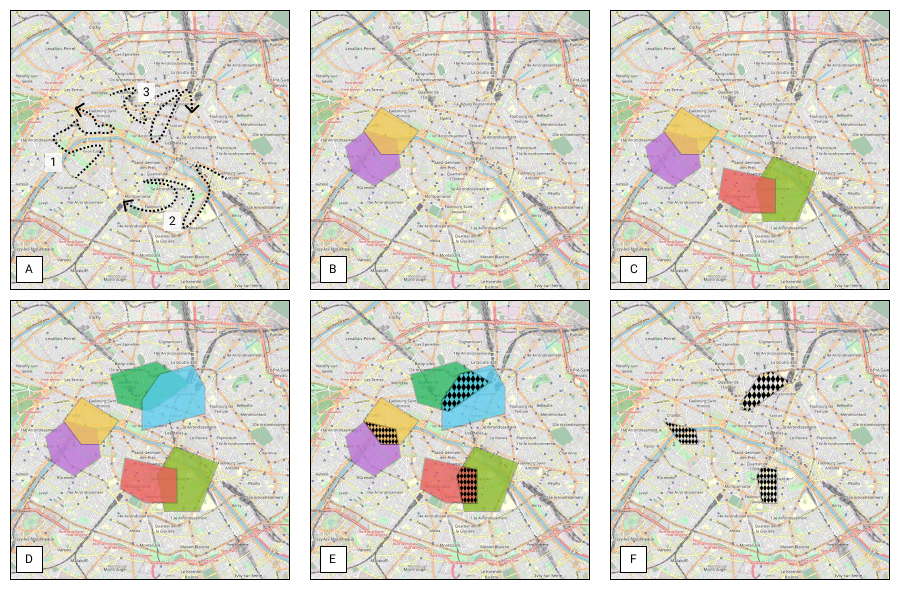
\includegraphics[width=\textwidth]{imagens/caso-de-estudo}
	\caption{Processo de explorar estadias em Paris}
	\label{fig:regions}
\end{figure}

{\bf Exemplo.} {\em Benício está planejando passar alguns dias em Paris, França. Sua apreciação pela cultura francesa faz com que ele tenha interesse em novas experiências na cidade. Ele decidiu por alugar uma estadia pelo Airbnb \footnote{\it http://www.airbnb.com}. Ele gosta de descobrir a cidade, portanto ele é aberto a qualquer tipo de estadia em qualquer região com um leve interesse em ficar perto do centro da cidade. O sistema retorna $4000$ opções diferentes. Como ele não tem outras preferências, é necessário uma investigação exaustiva para avaliar cada região da cidade independentemente, o que é quase impossível. Enquanto estava avaliando algumas opções, ele demonstrou interesse na região de  ``Champ de Mars'' (próximo à Torre Eiffel), mas esqueceu ou não achou necessário clicar num ponto nesta região. Coletando o feedback do seus movimentos com o mouse no mapa de estadias em Paris, a abordagem proposta consegue de maneira transparente detectar o interesse dele na região supracitada e apresentar uma quantidade pequena de opções recomendadas para Benício.}

O exemplo acima é usado para descrever como feedback implícito é coletado na prática. Imagem \ref{fig:regions} mostra os passos de Benício para explorar estadias em Paris. Imagem \ref{fig:regions}.A mostra os movimentos do mouse dele em diferentes intervalos de tempo. Nesse exemplo, o feedback de Benício é coletado em 3 diferentes intervalos de tempo (evoluindo das Imagens \ref{fig:regions}.B até \ref{fig:regions}.D). Isso mostra que Benício começou sua busca perto da Torre Eiffel e {\em Arc de Triomphe} (Imagem \ref{fig:regions}.B) e gradualmente mostrou também interesse no sul (Imagem \ref{fig:regions}.C) e norte (Imagem \ref{fig:regions}.D). Todas as interseções entre essas regiões são descobertas (regiões tachadas na Imagem \ref{fig:regions}.E), o que representa um conjunto de regiões onde o interesse de Benício está direcionado e onde, provavelmente, ele vai decidir ficar durante sua visita à Paris.

E se Benício quiser voltar para Paris próximo ano? Ele teria que repetir a mesma análise exploratória, a não ser que ele lembre a localização exata das estadias interessantes a ele no ano passado. Na abordagem proposta, ele não precisaria lembrar, porque suas preferências foram coletadas e poderiam ser usadas para realçar um subconjunto similar ao do ano anterior.

No contexto da análise exploratória, o analista talvez mude suas preferências entre as sessões (por exemplo, no inverno, Benício talvez queira ficar próximo à Torre Eiffel, mas no verão, ele talvez queira ficar mais distante dos pontos turísticos). A fim de enfrentar esse desafio, é proposto um modelo que permite uma análise de variação temporal para identificar padrões em como as preferências dos analistas mudam entre as sessões, o que permite aprimorar o método de realçamento para ser mais preciso e consistente com o interesse do analista mesmo em momentos diferentes do ano, por exemplo.

\section{Objetivos}

Nesta seção, define-se os objetivos gerais e específicos do trabalho.

\subsection{Objetivos Gerais}

\begin{itemize}
	\item Propor um modelo de análise espaço-temporal para orientação na exploração de dados espaciais;
	\item Elaborar como análise temporal pode ser efetivamente aplicada na exploração de dados espaciais.
\end{itemize}

\subsection{Objetivos Específicos}

\begin{itemize}
	\item Descrever o conceito de Regiões Densas Interessantes usado para captura de feedback;
	\item Apresentar como o modelo de dados pode ser aplicado no contexto da análise exploratória;
	\item Descrever o modelo de dados usado para análise temporal;
	\item Investigar como o modelo proposto pode ser explorado no contexto espacial e no contexto de domínio.
\end{itemize}

\section{Organização}

Os próximos capítulos estão organizados na seguinte maneira: no Capítulo \ref{chap:contextualizacao} é discutido o estado da arte por trás desse trabalho; Capítulo \ref{chap:modelo} define o modelo de dados, apresenta como é feito a coleta de feedback durante a análise exploratória e demonstra como a análise de variação temporal pode ser aplicada. Capítulo \ref{chap:conclusao} conclui e propõe futuros trabalhos.


\chapter{Contextualização}
\label{chap:contextualizacao}

Este capítulo dá uma visão geral sobre os trabalhos relacionados acerca de exploração de feedback, métodos de destacamento de informações e aplicação de análises temporais. Também é apresentado o sistema que está sendo estendido neste trabalho.

\section{Trabalhos Relacionados}

A literatura na análise de dados espaciais possui um foco na eficiência das iterações exploratórias. A abordagem comum é projetar índices pré-processados, os quais permitem a consulta eficiente de dados espaciais \cite{lins2013nanocubes}. No entanto, também é preciso direcionar a atenção para o {\em valor} dos dados espaciais, porque é muito comum encontrar um analista se perdendo numa enorme quantidade de pontos geográficos. Para solucionar esse problema, ambientes de visualização, como, por exemplo, Tableau\footnote{\it http://www.tableau.com}, Exhibit\footnote{\it http://www.simile-widgets.org/exhibit/}, Spotfire\footnote{\it  http://spotfire.tibco.com}, oferecem funcionalidades para manipular os dados como filtros, consultas agregadores, entre outras. Entretanto essas funcionalidades não se mostram eficazes, visto que nessas ferramentas o pesquisador precisa saber exatamente o que procura. Este trabalho combina a exploração de feedback, métodos de destacamento de informações e análise temporal a fim de otimizar a análise exploratória.

\subsection{Exploração de Feedback}

O modelo espaço-temporal proposto aprimora o processo de análise de dados espaciais destacando subconjuntos de pontos geográficos com base no feedback coletado durante a exploração do analista. Na literatura, há vários trabalhos sobre exploração de feedback para orientar o analista nas futuras iterações da análise como, por exemplo, \citeonline{boley2013one}. A abordagem comum é uma metodologia {\em top-$k$} para reduzir o escopo da consulta baseado no feedback explícito e recomendar um pequeno subconjunto de resultados interessantes de tamanho $k$. Uma clara distinção do presente trabalho é que não busca-se reduzir o escopo, mas alavancar o conjunto de dados com resultados potencialmente interessantes que o analista talvez não tenha notado devido ao enorme volume de dados espaciais. Enquanto as escolhas do analista são limitadas por $k$ em algoritmos de {\em top-$k$} processamento, a abordagem proposta oferece a liberdade de escolha ao mesmo tempo que pontos geográficos vão sendo transparentemente destacados com base nas novas escolhas do analista.

\subsection{Métodos de Destacamento de Informação}

\todo{fala de cada um}

Há trabalhos na literatura sobre métodos de destacamento de informações, por exemplo: \citeonline{Liang2010,Robinson2011,wongsuphasawat2016voyager,willett2007scented}. Entretanto todos esses métodos são {\em objetivos} e não são aplicáveis para o contexto de orientação espacial onde o feedback do usuário é envolvido. Em termos de recomendação, algumas abordagens focam na dimensão espacial \cite{Bao2015,Levandoski:2012} enquanto o contexto e a diversidade do resultado é deixado de lado.

\subsection{Aplicações de Análise Temporal}

Existem várias instâncias na literatura que combinam análise temporal com dados espaciais, como \citeonline{baculo2017,balahadia2017,chidean2018,ghahramani2018,kamath2013,lopestexeira2018,ma2017,mijovic2016,tomoki2010,nara2007,zhan2017,zheng2018}. Essas aplicações de análise temporal são em contextos específicos, os quais não envolvem feedback do usuário, mas representam como análise temporal pode ser perspicaz e proveitosa.

\citeonline{baculo2017} e \citeonline{balahadia2017} fazem uso de dados públicos de Manila, capital das Filipinas, combinando dados espaciais, análise temporal e modelos preditivos e mostrando resultados que podem ser utilizados para preparação de um plano de gestão pública eficaz. \citeonline{ma2017} e \citeonline{zheng2018} também fazem análises realistas de como eventos, como protestos, impactam nas trajetórias de táxis, cujos resultados podem auxiliar no controle de tráfego urbano e nos planos de serviços de transporte da cidade. Ambos realizam ricas análises, as quais contribuíram como inspiração neste trabalho.

\citeonline{chidean2018} apresenta como detectar padrões espaço-temporais no contexto do uso de energia eólica na Península Ibérica usando o algoritmo {\em Second-Order Data-Coupled Clustering}. Apesar do estudo detalhado, esse trabalho não contempla um contexto de análise exploratória.

\citeonline{ghahramani2018}, \citeonline{lopestexeira2018} e \citeonline{zhan2017} demonstram como análise temporal pode ser aplicada no contexto geográfico. \citeonline{zhan2017} vai além gerando uma árvore de clusterização hierárquica. Apesar dos métodos e resultados serem bem detalhados nos trabalhos, essas contribuições não se aplicam ao assunto em questão.

\citeonline{kamath2013} propõe uma abordagem de {\em reinforcement learning} para prever eventos (adoção de {\em memes}) num contexto espaço-temporal. \citeonline{nara2007} introduz um modelo de visualização 3D para dados espaço-temporais que ajuda a analisar qualitativa e quantitativamente os padrões e tendências espaço-temporais. Ambos os trabalhos contribuem para representar como o modelo proposto pode ser combinado com diversas técnicas.

\section{GeoGuide}

\begin{figure}[t]
	\centering
	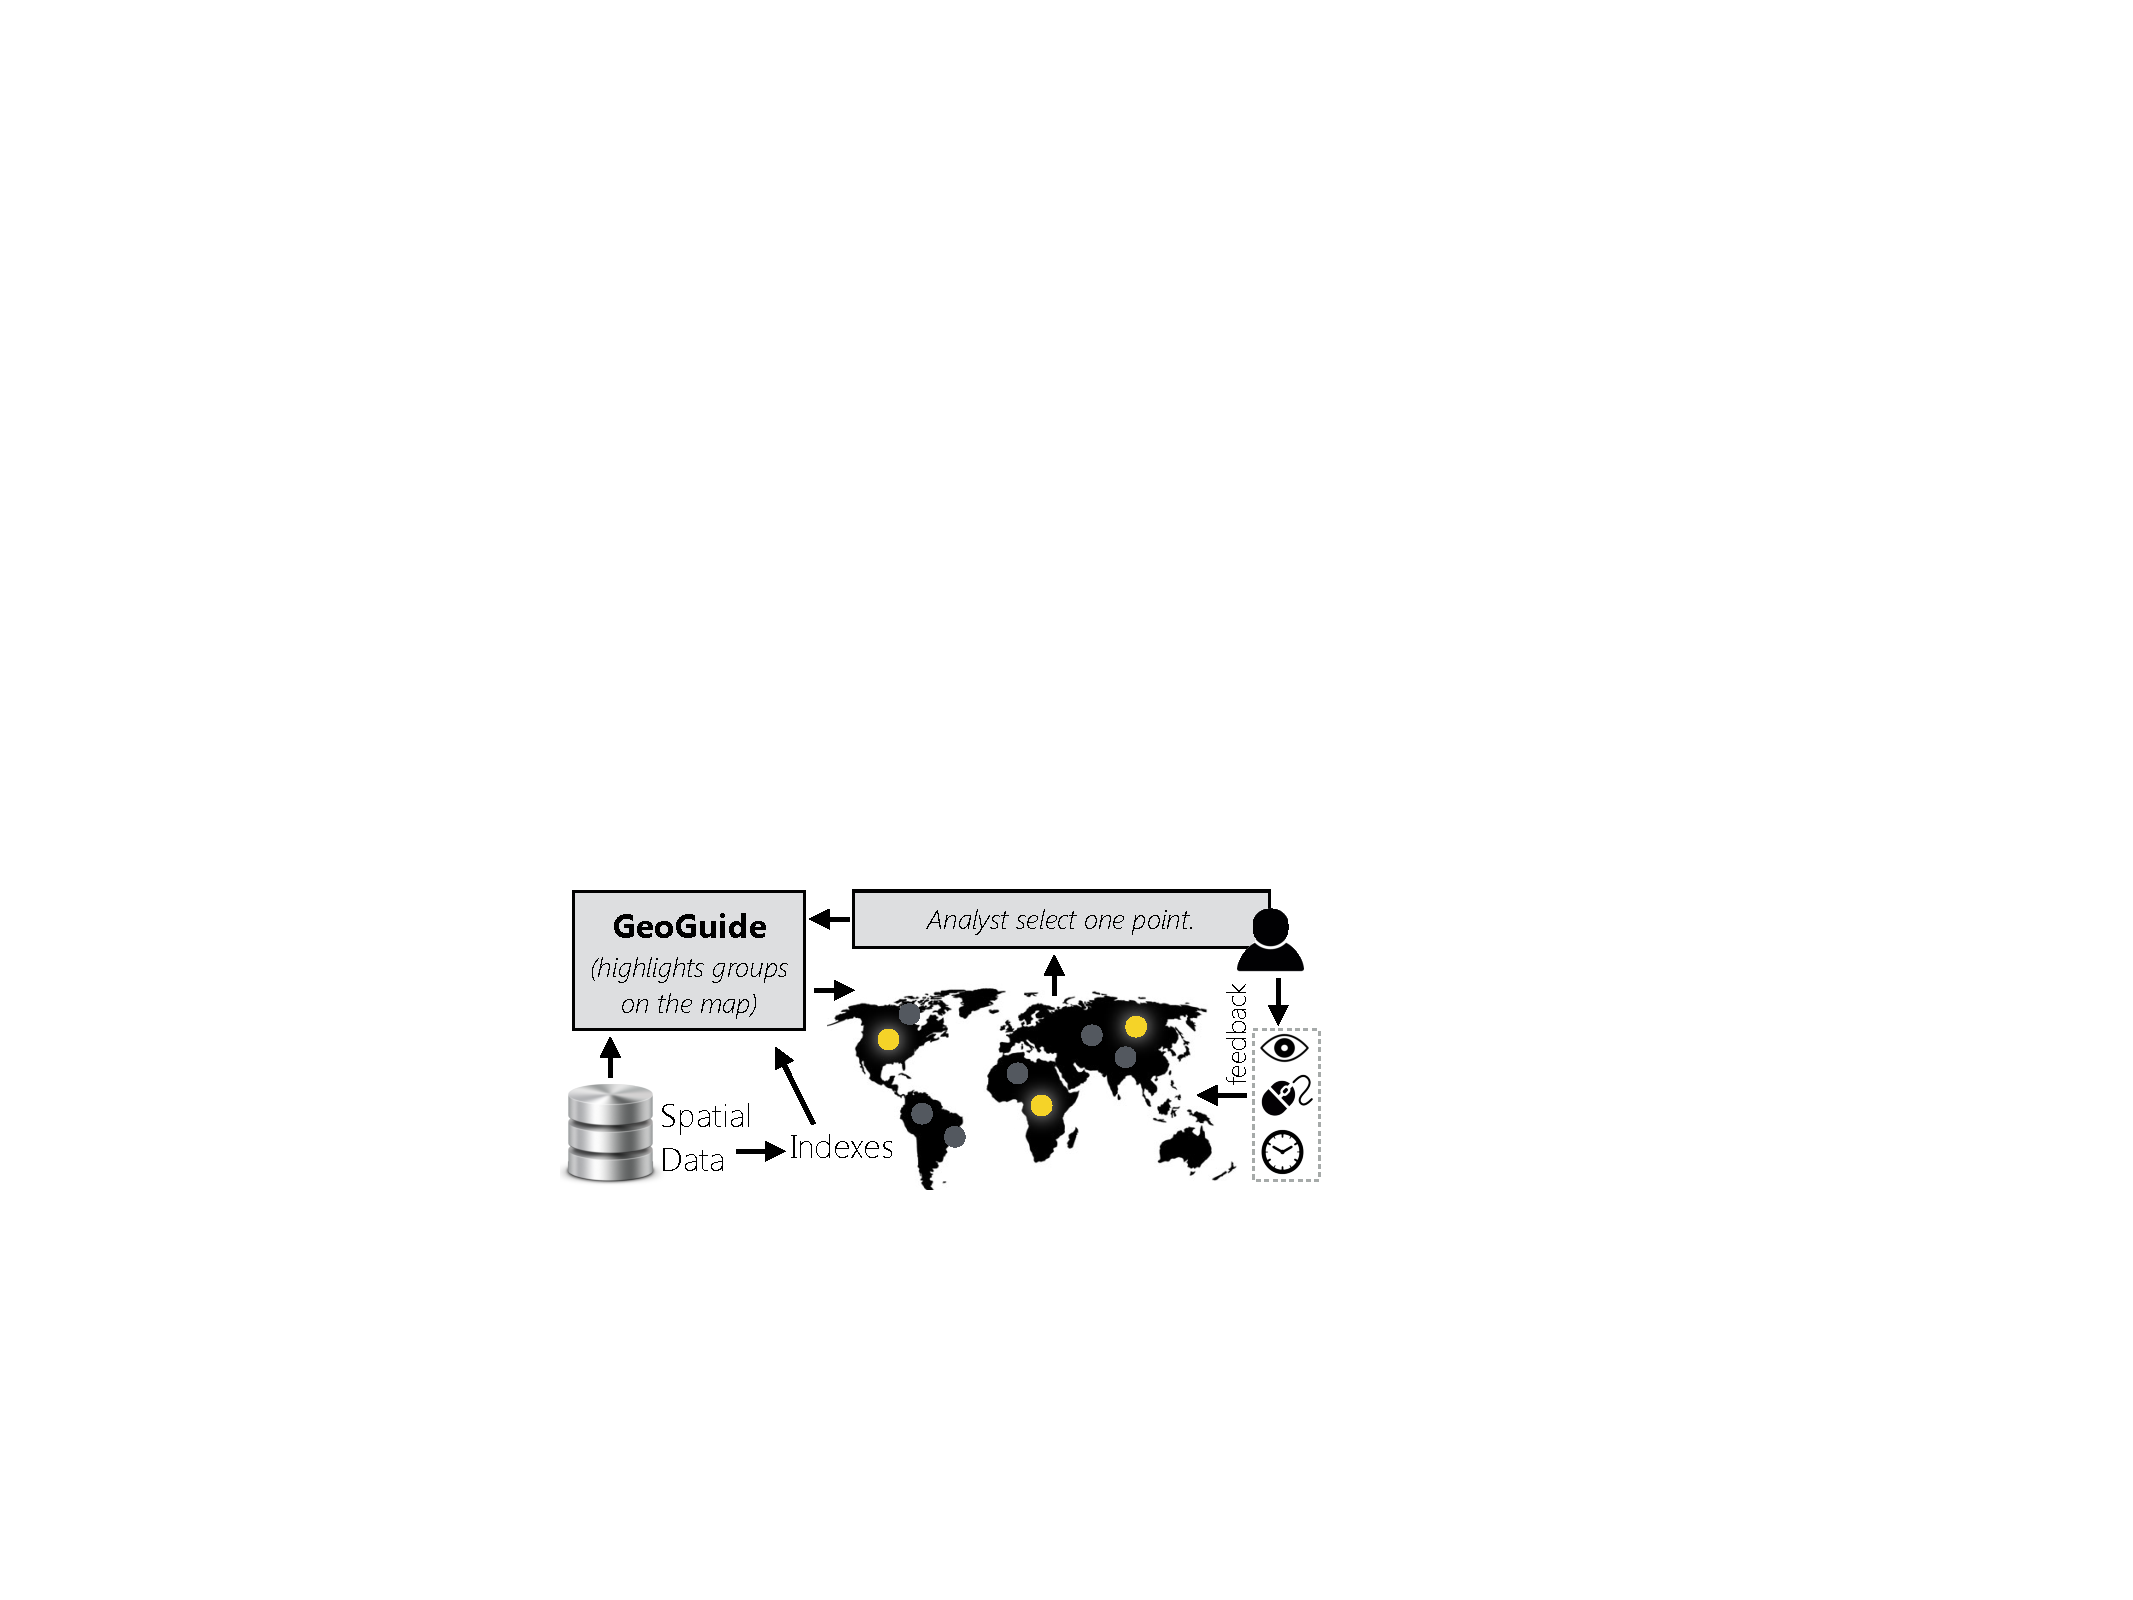
\includegraphics[width=\columnwidth]{imagens/framework}
	\caption{Componentes do GeoGuide}
	\label{fig:framework}
	\vspace{-10pt}
\end{figure}

\abrv[TADS -- Tecnologia em Análise e Desenvolvimento de Sistemas]{}
\abrv[IFRN -- Instituto Federal do Rio Grande do Norte]{}

GeoGuide \cite{omidvarTehrani2017} é fruto de um projeto de pesquisa realizado por alunos do curso de Tecnologia em Análise e Desenvolvimento de Sistemas (TADS) no Instituto Federal do Rio Grande do Norte (IFRN) em colaboração com a Universidade de Grenoble. Esse projeto se trata de um ambiente de visualização de dados espaciais que coleta as preferências do usuário durante a exploração para destacar subconjuntos de pontos geográficos que podem ser interessantes ao analista. Figura \ref{fig:framework} ilustra os principais componentes da arquitetura do GeoGuide explorados nas próximas subseções.

Neste trabalho, o GeoGuide é potencializado à dois novos conceitos: $i$. regiões densas interessantes e $ii$. análise temporal das preferências do usuário. Esses dois conceitos serão explorados no próximo capítulo.

\subsection{Pré-processamento}

GeoGuide realiza um passo de pré-processamento para criar os índices que serão usados durante a fase de destacamento. O índice é uma tabela comparativa entre todos os pontos usando duas métricas de qualidade: relevância e diversidade. Os valores calculados são normalizados no intervalo de $0.0$ à $1.0$.

\subsubsection{Relevância e Diversidade}

\begin{figure}[t]
	\centering
	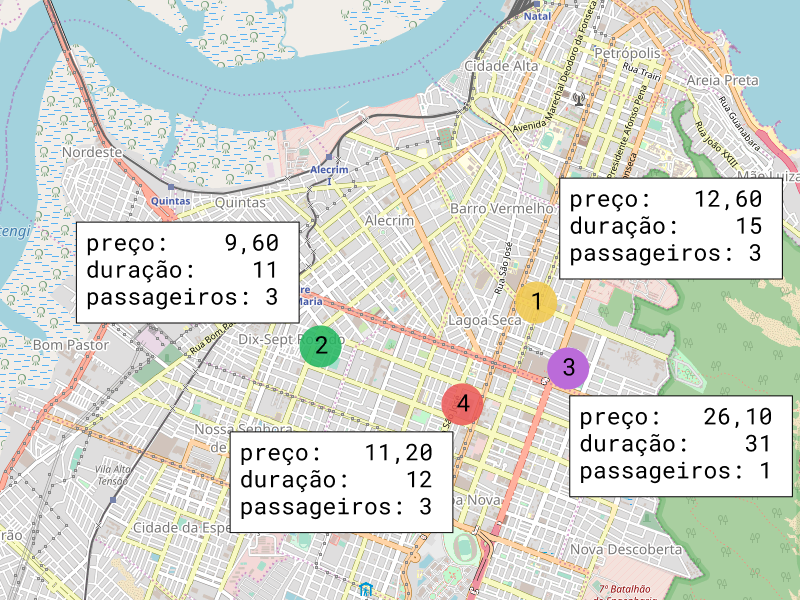
\includegraphics[width=\columnwidth]{imagens/exemplo-de-pontos}
	\caption{Exemplo de pontos geográficos com seus atributos}
	\label{fig:exemplo-pontos}
	\vspace{-10pt}
\end{figure}

Relevância representa o quão similar é o ponto $a$ com o ponto $b$ num conjunto de dados. GeoGuide usa a relevância para destacar pontos similares ao feedback do analista. Diversidade representa quão distante o ponto $a$ está localizado do ponto $b$. GeoGuide usa a diversidade para permitir ao analista explorar diferentes regiões, mas ainda assim trabalhar com pontos relevantes ao seu interesse.

\begin{table}[!h]
	\centering
	\begin{tabular}{|c|c|r|r|}
	\hline
	\multicolumn{1}{|c|}{\textbf{Ponto A}} & \multicolumn{1}{c|}{\textbf{Ponto B}} & \multicolumn{1}{c|}{\textbf{Relevância}} & \multicolumn{1}{c|}{\textbf{Diversidade}} \\ \hline
	1                                      & 2                                     & 0.8                                      & 0.9                                       \\ \hline
	1                                      & 3                                     & 0.25                                     & 0.2                                       \\ \hline
	1                                      & 4                                     & 0.9                                      & 0.45                                      \\ \hline
	2                                      & 3                                     & 0.2                                      & 1.0                                       \\ \hline
	2                                      & 4                                     & 1.0                                      & 0.48                                      \\ \hline
	3                                      & 4                                     & 0.2                                      & 0.3                                       \\ \hline
	\end{tabular}
	\caption{Exemplo de Índice de Relevância e Diversidade para pontos na Figura \ref{fig:exemplo-pontos}}
	\label{table:exemplo-indice}
\end{table}

Na Figura \ref{fig:exemplo-pontos}, tem-se, por exemplo, pontos geográficos que representam viagens de táxi. Cada ponto (1, 2, 3 e 4), possui seus atributos: preço da viagem, duração da viagem e a quantidade de passageiros; e sua localização geográfica. Na tabela \ref{table:exemplo-indice}, ilustra-se o exemplo do índice calculado diante dos pontos apresentados na Figura \ref{fig:exemplo-pontos}. Percebe-se que os pontos mais similares entre si são os pontos 2 e 4, enquanto que 2 e 3 são os mais distantes, ou seja, possuem o maior valor de diversidade.


\subsection{Preferências do Usuário}

Para coletar as preferências do usuário, GeoGuide usa ambos feedback implícito e explícito. Feedback explícito é quando o usuário está analisando os atributos de um ponto, por exemplo a descrição de uma casa no Airbnb, e explicitamente pede para explorar pontos similares ao selecionado. Feedback implícito é coletado através da captura dos movimentos do mouse e métricas como  ``quanto tempo o usuário passou analisando o perfil de um ponto''.

\subsection{Destacamento de Dados Espaciais}

GeoGuide combina o índice pré-processado e o feedback coletado para destacar subconjuntos de dados espaciais de acordo com as preferências do analista. O processo de destacamento provou ser eficiente em termos de ``quantos passos o analista leva até completar a tarefa de encontrar um ponto com um determinado perfil''. Usando GeoGuide, analistas foram capazes de completar a tarefa usando, em média, 10.7 passos, enquanto que usando Tableau, foram necessários 43 passos \cite{omidvarTehrani2017}.

% \vspace{25pt}
% \endsubsection

% \closesubsection


\chapter{Definição do Modelo}
\label{chap:modelo}

Neste capítulo, entendemos as Regiões Densas Interessantes e definimos o modelo espaço-temporal.

\section{Regiões Densas Interessantes}

Uma Região Densa Interessante (IDR, do inglês \em{Interesting Dense Region}) é uma região espacial com uma alta probabilidade de conter pontos de interesse do analista. IDR são coletadas e definidas durante o processamento do feedback do usuário. Diferentemente da literatura que predominantemente foca em intereções explícitos (como clicar no botão, abrir o perfil do ponto), investigamos o feedback implícito.

Durante a exploração iterativa de dados espaciais, é comum o caso que o analista avalia algumas regiões de interesse, mas esquece de dá um feedback explícito sobre aquela região. O ato do usuário olhar para essa região pode ser capturado através do rastreio da movimentos oculares e, como \citeonline{arapakis2014user} mostra, esse método possui uma forte relação com a atenção do usuário.

Entretanto o rastreamento dos movimentos oculares fere várias questões de privacidade, assim sendo optamos pela alternativa de rastrear os deslocamentos do cursor do mouse. \citeonline{arapakis2014understanding} argumenta que esse método possui uma forte relação com o engajamento do usuário. Intuitivamente, um ponto espacial recebe um feedback positivo se o cursor do mouse se desloca próximo a ele frequentemente.

Continua...

\section{Spatial layer}

Each point in a dataset ($p \in \mathcal{P}$) is described using its coordinates (latitude and longitude) and also associated with a set of attributes ($dom(p)$). For instance, TODO

\section{Interesting Dense Regions}

TODO

We have IDRs per iteration/session where implicit feedback is captured such mouse moves (or eye gaze). In the beginning, each IDRs is a group of raw points described using its coordinates (latitude and longitude) and a timestamp (the unix timestamp it was captured). These raw points once captured will enter the clustering (for now, ST-DBSCAN) phase to generate the IDR itself with a profile. The profile is built based on the spatial layer and it should represent a summary of its contained points from the spatial layer.

\begin{itemize}
	\item A profile has summary of its spatial points number attributes. For each number attribute in $dom(p)$, we calculate the average, median and standard deviation based on the points contained in the IDR.

	\item A profile has a word rank $R$ of the terms in the text attributes of its spatial points. For each text attribute in $dom(p)$, we evaluate the most used terms in order to create a word rank \cite{kumar2017}.

	\item A profile has a map $M$ between the $<name, value>$ of categoricals attributes and its relevance in $dom(p)$.

	\item TODO: datetime attributes

	\item A profile has a meta property with values such the count of points in the IDR.
\end{itemize}

\section{Highlighting}

TODO

% \chapter{Coletando Feedback}
\label{chap:coletando}

TODO

% \chapter{Aplicando Análise Temporal}
\label{chap:aplicando}

TODO

% \chapter{Guiando o Usuário}
\label{chap:guiando}

Neste capítulo, entendemos como combinamos o feedback coletado com a aplicação da análise temporal para guiar o analista durante as iterações da análise exploratória.

\section{Destacamento de Informação}

Utilizamos o método de destacamento de informação para guiar o usuário.

Aprimoramos o algoritmo IUGA... explicação do algoritmo.

% \chapter{Experimentos}
\label{chap:experimentos}

TODO

\section{Resultados}

TODO

\chapter{Considerações Finais}
\label{chap:conclusao}

Neste trabalho é proposto um modelo de análise espaço-temporal para identificação de padrões nas preferências coletadas pela ferramenta GeoGuide enquanto um analista realiza a análise exploratória de dados espaciais. O modelo proposto mostra-se viável para ser utilizado a fim de aprimorar o uso da captura de {\em feedback} implícito para orientar o usuário nas próximas iterações através do método de destacamento de pontos geográficos.

\section{Contribuições}

O modelo propõe 2 novos conceitos: $i$. regiões densas interessantes e $ii$. análise temporal das preferências do usuário. As regiões densas interessantes (IDR) representam as preferências do analista no contexto espacial no determinado momento. Cada IDR possui também um perfil que representa as preferências do analista no contexto de domínio.

As regiões e seus perfis permitem a análise temporal das preferências do usuário. Os métodos para análise em ambos contextos espaciais e de domínio são investigados e apresentados com o propósito de identificar padrões nas iterações da análise exploratória.

\section{Trabalhos futuros}

Os dados gerados pelo modelo proposto podem futuramente ser explorados em diversos cenários. Por exemplo, os dados gerados podem ser utilizados para entender as preferências de um grupo de analistas a fim de potencializar o descobrimento de objetivos comuns entre eles.

No que diz respeito aos ambientes de exploração de dados espaciais, os dados coletados podem ser combinados com algoritmos preditivos para responder questionamentos como ``onde o analista deve está interessado na próxima iteração?'' ou até mesmo ``será que o analista está interessado neste apartamento com varanda?''.  

% Bibliografia (arquivo Capitulos/Referencias.bib)

\bibliography{capitulos/referencias}
\bibliographystyle{abnt-alf}

% Ap���ndice A (arquivo Includes/ApendiceA)
% \include{capitulos/ApendiceA}

% Anexo A (arquivo Includes/AnexoA)
% \include{capitulos/AnexoA}

% P���gina em branco
\newpage

\end{document}